\documentclass[./../../paper.tex]{subfiles}
\graphicspath{{\subfix{./../../figures/}}}

\begin{document}

\section{Determine the best Generator Algorithm}

\subsection{Experimental Setup}
\label{sec:exp4}
Knowing the , we compare the evolutionary algorithm with other algorithms. 

In this comparison, we employ the other models mentioned in \autoref{sec:models}. Namely, the \emph{Case-Based Generator} and the \emph{Random Generator}. 

For the evolutionary algorithm, we choose the model-configuration from \autoref{sec:exp1}, the rate-configuration determined in \autoref{sec:exp2} and the termination point from \autoref{sec:exp3}. Furthermore, we randomly sample \attention{20} factuals from the test set and use the same factuals for every generator. We ensure, that the outcomes are evenly divided. The remaining procedure follows the established procedure of previous experiments.

\subsection{Results}
\begin{figure}[htbp]
    \centering
    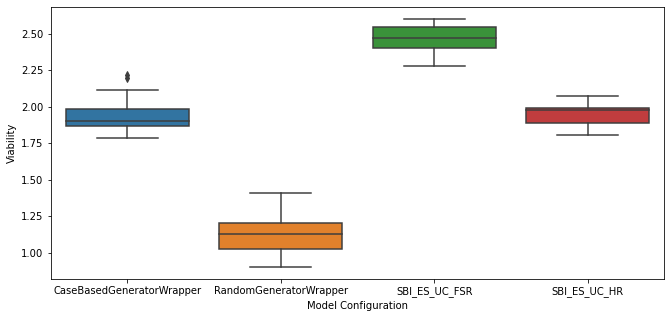
\includegraphics[width=\textwidth]{figures/generated/exp4_winner_figure_side.png}
    \caption{This figure shows boxplots of the viability of each models' generated counterfactual.}
    \label{fig:exp4-winner}
\end{figure}

\noindent the results shown in \autoref{fig:exp4-winner} indicate that in terms of our viability measure, the evolutionary model returns better counterfactuals than othe baselines. 

\autoref{tbl:exp4-winner} shows the detailed results.

\begin{table}
\caption{shows the result the average Viability for each model.}
\label{tbl:exp4-winner1}
\begin{tabular}{lrrrrr}
 & Similarity & Sparcity & Feasibility & Delta & Viability \\
Model Configuration &  &  &  &  &  \\
CaseBasedGeneratorWrapper & 0.774812 & 0.590326 & 0.032561 & 0.550288 & 1.947988 \\
RandomGeneratorWrapper & 0.407410 & 0.188083 & 0.000000 & 0.535299 & 1.130793 \\
SBI-ES-UC-FSR & 0.753882 & 0.615751 & 0.102992 & 0.996515 & 2.469140 \\
SBI-ES-UC-HR & 0.645248 & 0.485620 & 0.000010 & 0.815731 & 1.946608 \\
\end{tabular}
\end{table}



\subsection{Discussion}
These results show that the model \attention{SBI-ES-OPC-FSR} is clearly superior to the other models. This result is unsurprising, as the baselines do not actively search for an optimal solution. However, knowing these results, a couple of questions remain. Namely, does the result remain consistent for longer sequences and does the result remain consistent for other datasets? \optional{Furthermore, how does this procedure compare to other methods in the literature?} The remaining experiments will address these issues. 


\end{document}